%%%%%%%%%%%%%%%%%%%%%%%%%%%%%%%%%%%%%%%%%
% a0poster Portrait Poster
% LaTeX Template
% Version 1.0 (22/06/13)
%
% The a0poster class was created by:
% Gerlinde Kettl and Matthias Weiser (tex@kettl.de)
% 
% This template has been downloaded from:
% http://www.LaTeXTemplates.com
%
% License:
% CC BY-NC-SA 3.0 (http://creativecommons.org/licenses/by-nc-sa/3.0/)
%
%%%%%%%%%%%%%%%%%%%%%%%%%%%%%%%%%%%%%%%%%

%-----------------------------------------------------------------------------
%	PACKAGES AND OTHER DOCUMENT CONFIGURATIONS
%-----------------------------------------------------------------------------
\pdfminorversion=4
\documentclass[a0,portrait]{a0poster}

%% % sans-serif config:


\usepackage[english]{babel}
\usepackage[utf8]{inputenc}
\usepackage[T1]{fontenc}
\renewcommand{\familydefault}{\sfdefault}

\usepackage{enumitem}

\usepackage{multicol} % This is so we can have multiple columns of
                      % text side-by-side
\columnsep=100pt % This is the amount of white space between the
                 % columns in the poster
\columnseprule=3pt % This is the thickness of the black line between
                   % the columns in the poster

\usepackage[svgnames]{xcolor} % Specify colors by their 'svgnames',
                              % for a full list of all colors
                              % available see here:
                              % http://www.latextemplates.com/svgnames-colors

\usepackage{tgheros}


%% \usepackage{times} % Use the times font
%% \usepackage{palatino} % Uncomment to use the Palatino fon

\usepackage{graphicx} % Required for including images
\usepackage{overpic}
\graphicspath{{figures/}} % Location of the graphics files
\usepackage{booktabs} % Top and bottom rules for table
\usepackage[font=small,labelfont=bf, format=hang]{caption} % Required for
                                              % specifying captions to
                                              % tables and figures
\usepackage{amsfonts, amsmath, amsthm, amssymb} % For math fonts,
                                                % symbols and
                                                % environments
\usepackage{wrapfig} % Allows wrapping text around tables and figures

%\usepackage{sfmath}
\usepackage[eulergreek]{sansmath} %additional math
\sansmath

\usepackage{mathsetup}

\usepackage{bibconfig}

\usepackage{titlesec}

\usepackage{siunitx}
\sisetup{detect-all}

\titlespacing*{\section}
{0pt}{2.5ex plus 1ex minus .2ex}{1.5ex plus .2ex}


\makeatletter
\g@addto@macro\normalsize{%
  \setlength\abovedisplayskip{18pt}
  \setlength\belowdisplayskip{18pt}
  \setlength\abovedisplayshortskip{16pt}
  \setlength\belowdisplayshortskip{16pt}
}
\makeatother


\addtolength{\parskip}{0.5\baselineskip}
\parindent 0pt

\definecolor{gblue}{RGB}{27,98,183}

\begin{document}

%-----------------------------------------------------------------------------
%	POSTER HEADER 
%-----------------------------------------------------------------------------

\vspace{-7cm}

\begin{minipage}[b]{0.9\linewidth}
  \veryHuge %
  \textbf{Nonrandom connectivity in local cortical circuits
          from anisotropic axon morphology} \color{Black}
\end{minipage}\\
%
\begin{minipage}[b]{0.5\linewidth}
  %       
  \vspace{1.5cm}
  %
  \huge \textbf{Felix Z. Hoffmann$^{1,2}$, Stefan Rotter$^{1,3}$}\\[0.9cm] 
  %
  \large $\quad ^1\,$Bernstein Center Freiburg, Freiburg, Germany\\[0.2cm]
  %
  $\quad ^2\,$Frankfurt Institute for Advanced Studies, Frankfurt am Main,
  Germany\\[0.2cm]
  %
  $\quad ^2\,$Faculty of Biology, University of Freiburg, Freiburg,
  Germany\\[-0.5cm]

\end{minipage}
%
%
\begin{minipage}[b]{0.5\linewidth}
  \centering
  
  %% 
\includegraphics[width=10cm]{goethe-logo.pdf}\\
  %% \vspace{2.8cm}
  \vspace{-4.2cm}
  
\includegraphics[width=7cm]{bcf_logo_2000.png} \hspace{3cm}
  
\includegraphics[width=11cm]{spp2041_logo.pdf}
  \vspace{1.2cm}
  \hspace{3cm}
         
\includegraphics[width=7cm]{wosf_tiny.png}     
    \vspace{0.5cm}


    \Large \texttt{hoffmann@fias.uni-frankfurt.de} %% \hspace{2cm} 
\includegraphics[width=2cm]{camok.jpg}
      \vspace{1.2cm}
      
\end{minipage}


%-----------------------------------------------------------------------------

\begin{multicols}{2}

  \section{Introduction}
\vspace{-0.2cm}

Experimental results indicate that connectivity in cortical circuits is highly nonrandom:
\begin{enumerate}[leftmargin=2cm]
  \itemsep0pt
\item Reciprocally connected pairs appear more often than expected by chance \cite{Song2005, Perin2011}
\item Certain triplet motifs of neurons are strongly overrepresented \cite{Song2005}
  \item Clusters of neurons show more often a high degree of connectivity than predicted from spatial connectivity \cite{Perin2011}
  \end{enumerate}

Recently, these characteristics have been found in detailed reconstructions of cortical circuits \cite{Gal2017} and it was shown that generic network models can account for some of these features \cite{vegue2017}. However, it remains unclear what properties of a cortical circuit affect the connectivity such that the structures above emerge. Here we propose a simple network model based on the stereotypical anisotropy of axon morphology (Fig.~\ref{fig:morphaniso}).

\begin{center}\vspace{0.01cm}
  \includegraphics[width=1.0\columnwidth]{%
    /home/fh/sci/rsc/aniso_netw/pub/arxiv18/figures/morphological_anisotropy/morphological_anisotropy_horizontal.pdf}
  \captionof{figure}{Projections of thick-tufted layer V pyramidal
cells in the rat somatosensory cortex (manually traced from \cite{Romand2011}) \textbf{A} Axon morphology of a single cell (left), branch density heatmap of axons for 5 neurons. \textbf{B} As in A, but for dendrite.}
  \label{fig:morphaniso}
\end{center}\vspace{2cm}


  
\vspace{-1.5cm}
\section*{Model}
\vspace{-0.2cm}

Motivated from the observed anisotropy in axonal morphology (Fig.~\ref{fig:morphaniso}) we formulate the \textit{anisotropic network model}: $N=1000$ neurons are distributed uniformly on a square of length \SI{296}{\micro\meter}. Each neuron is assigned a random direction $\alpha \in [0,2\pi)$ and connections are established to target neurons lying within in a corridor of width $w=\text{\SI{74.6}{\micro\meter}}$ (Fig.~\ref{fig:4nets}A). Here, the width $w$ was tuned to obtain a network connection density of $p=0.116$ as found in \cite{Song2005}.

\begin{center}\vspace{0.3cm}
  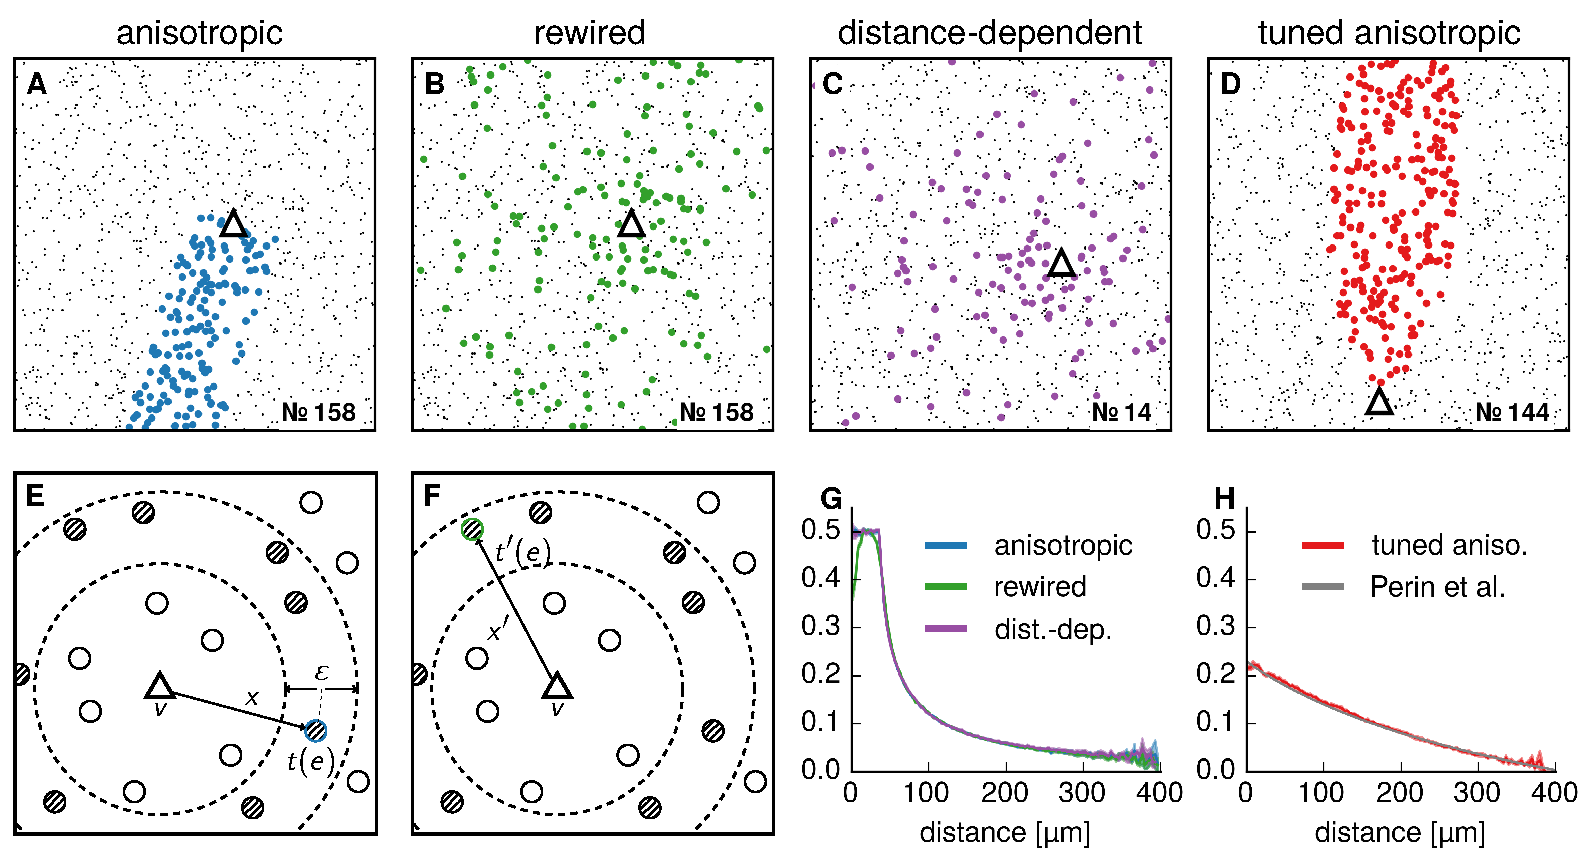
\includegraphics[width=\columnwidth]{%
    /home/fh/sci/rsc/aniso_netw/pub/arxiv18/figures/4_network_models/4_network_models.pdf}
  \captionof{figure}{Network models. \textbf{A-D} Targets of a single neuron (Id in bottom right corner) for the different network models \textbf{E-F} Rewiring algorithm. \textbf{G-H} Distance-dependent connection probabilities.}
  \label{fig:4nets}
\end{center}\vspace{2cm}

The \textit{rewired network} (Fig.~\ref{fig:4nets}B) is obtained from the anisotropic network by randomly picking new targets that differ in distance to the source neuron maximally by $\epsilon$ from the original target (Fig.~\ref{fig:4nets}E-F). The \textit{distance-dependent network} (Fig.~\ref{fig:4nets}C) is a randomly connected graph where the probability of a connection to exist depends on the distance between the nodes, using for example the profile of the anisotropic network (Fig.~\ref{fig:4nets}G). Finally, the \textit{tuned anisotropic network} (Fig.~\ref{fig:4nets}D) is similar to the anisotropic network with the difference that the corridor is shaped in such a way that the distance-dependent connection probability found in \cite{Perin2011} is obtained in the network (Fig.~\ref{fig:4nets}H).




  
\vspace{-0.5cm}
\section*{Results}
\vspace{-0.5cm}

In both anisotropic and tuned anisotropic networks, reciprocally
connected pairs occur more often than in a random network with the
same connection density (Fig.~\ref{fig:2neuron1}A).

\begin{center}\vspace{0.01cm}
  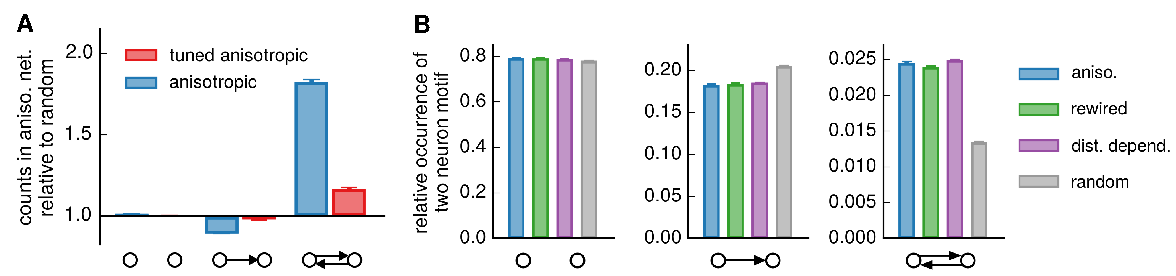
\includegraphics[width=\columnwidth]{%
    figures/two_neuron_figure_part1.pdf}
  \captionof{figure}{Unconnected, unidirectional and bidirectional
    neuron pair occurrences in the network models}
  \label{fig:2neuron1}
\end{center}\vspace{2cm}

However, is this due to anisotropy? Indeed, we find almost identical
pair counts in rewired and distance-dependent networks
(Fig.~\ref{fig:2neuron1}B). The overrepresentation of reciprocal
connections in the data of Perin et al.~\cite{Perin2011} is not
explained by distance-dependency, so that there could be other
pair-symmetric irregularities in the connection probabilities that
cause the overrepresentation \cite{Hoffmann2017}.

% \begin{center}\vspace{0.01cm}
%   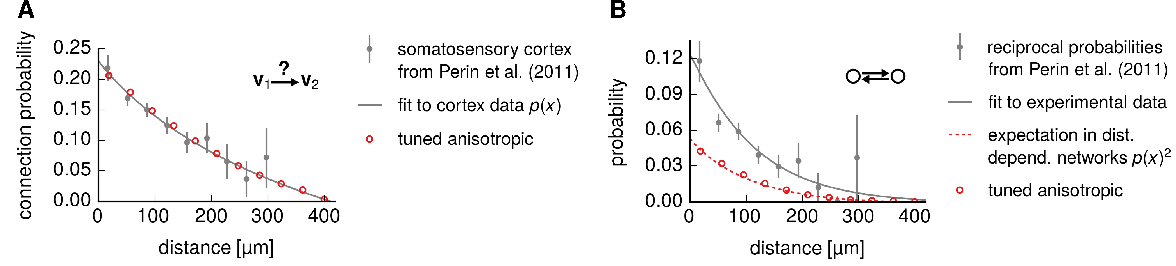
\includegraphics[width=\columnwidth]{%
%     figures/two_neuron_figure_part2.pdf}
%   \captionof{figure}{Distance-dependent probability of connection
%     (\textbf{A}) and probability of a reciprocal connection
%     (\textbf{B}).}
%   \label{fig:2neuron2}
% \end{center}\vspace{1.6cm}

Next we tested the occurrence of three neuron patterns as reported in
\cite{Song2005}. We found that in alignment with experimental results,
certain motifs are strongly overrepresented in the anisotropic
networks (Fig.~\ref{fig:3neuron}). Here, it is indeed anisotropy that
causes the motifs to appear more often -- the motif
overrepresentations are drastically reduced in rewired and
distance-dependent
networks.  %% In particular, motifs 4, 10, 12 and 14 were also reported in \cite{Perin2011} to be overrepresented.

\begin{center}\vspace{0.01cm}
  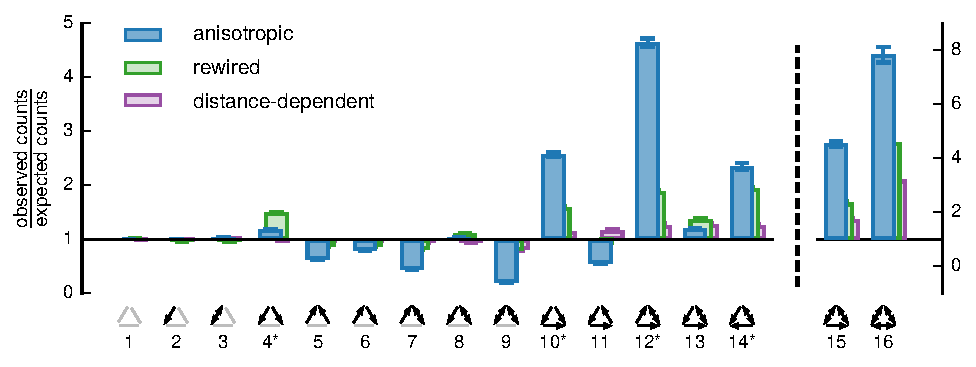
\includegraphics[width=\columnwidth]{%
    figures/fig4_3motif_aniso-rew-dist.pdf}
  \captionof{figure}{Occurrence of three neuron patterns relative to
    expected counts from pair statistics. Motifs indexed with * were
    reported to be overrepresented in \cite{Perin2011}.}
  \label{fig:3neuron}
\end{center}\vspace{2cm}

Perin et al.~\cite{Perin2011} reported that in somatosenory cortex of
rats, groups of neurons more often show a high connection density than
expected from the measured distance-dependent connection
probabilities. Both anisotropic and tuned anisotropic networks also
showed this effect in groups of 3, 6, 8 and 12 cells
(Fig.~\ref{fig:clusters}).

\begin{center}\vspace{0.01cm}
  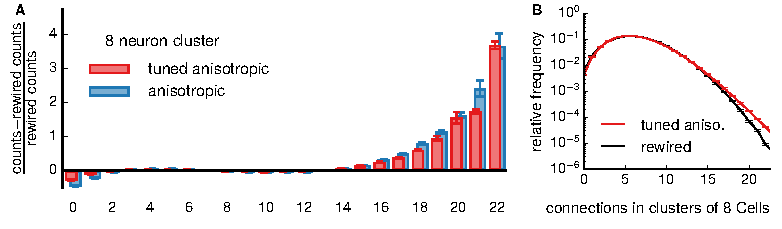
\includegraphics[width=\columnwidth]{%
    figures/nc2_8c-8f.pdf} \captionof{figure}{For groups of 8 cells a
    high number of connections appears more often in anisotropic and
    tuned anisotropic networks than in their rewired
    versions. \textbf{A} Relative difference in occurrence.
    \textbf{B} Frequency of number of connections in tuned anisotropic
    networks and their rewired version.}
  \label{fig:clusters}
\end{center}\vspace{2cm}

What other network connectivity properties does anisotropy affect? By
only partially rewiring anisotropic networks, we found that the
distribution of shared inputs to a random pair of neurons is shaped by
anisotropy (Fig.~\ref{fig:rewcom}A-C). In anisotropic networks
unconnected, unidirectionally connected and reciprocally connected
neuron pairs have distinctly different in-neighbour distributions,
which is not the case for distance-dependent networks
(Fig.~\ref{fig:rewcom}D-E).

\begin{center}\vspace{0.01cm}
  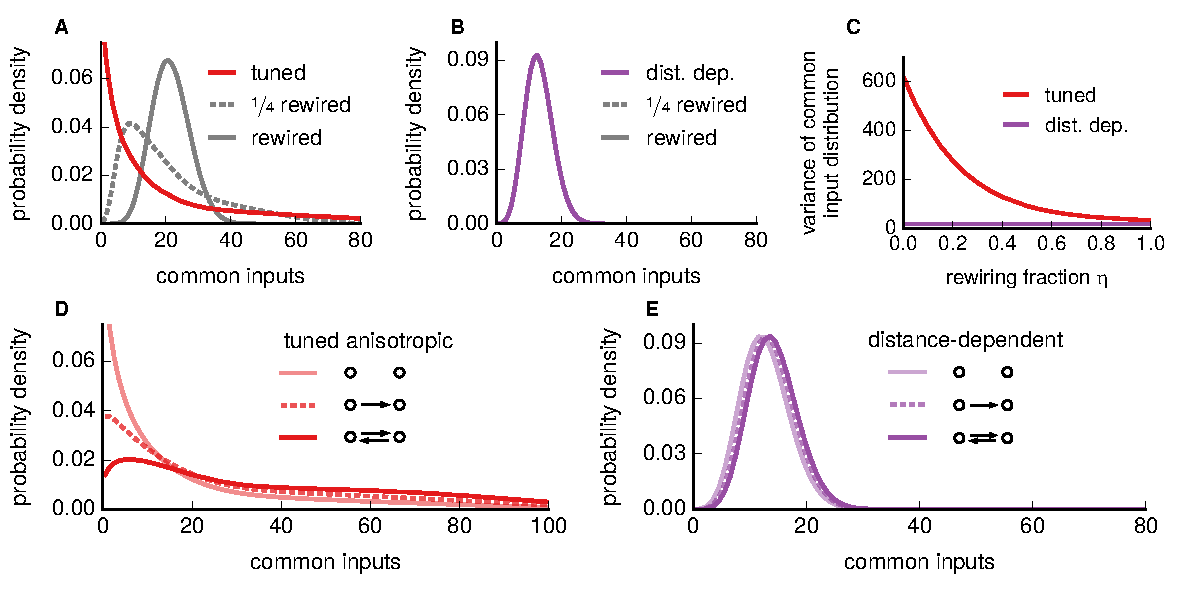
\includegraphics[width=\columnwidth]{%
    figures/fig6.pdf} \captionof{figure}{Anisotropy in spatial
    connectivity affects the distribution of common inputs. \textbf{A}
    Common in-neighbours to a random neuron pair in tuned anisotropic
    networks, partially rewired networks and fully rewired
    networks. \textbf{B} Common in-neighbour distribution in
    distance-dependent networks and rewired versions. \textbf{C}
    Variance of common in-neighbour distribution in tuned anisotropic
    and distance-dependent networks as a function of rewiring
    fraction. \textbf{D-E} Common input distribution of unconnected,
    unidirectionally and bidirectionally connected neuron pairs in
    anisotropic tuned and distance-dependent networks.}
  \label{fig:rewcom}
\end{center}\vspace{2cm}

\vspace{-1.25cm}
\section*{Key points}
\vspace{-0.5cm}
\begin{itemize}[leftmargin=1.3cm]
\item[-] Anisotropy in spatial connectivity as result of stereotypical
  anisotropy in axon morphology
\item[-] Nonrandom connectivity patterns identified in anisotropic
  network model suggest that prominent connectivity structures of cortical
  circuits might arise from neuron morphology
\item[-] Common input statistics particularly affected by anisotropy:
  Induces broad distributions and significant differences between
  connected and unconnected neuron pairs
\end{itemize}

\bigskip






  
\section*{Key points}
\vspace{-0.1cm}

\vspace{15cm}


  \printbibliography  

\end{multicols}

\end{document}
